\documentclass[10pt,conference,a4paper]{IEEEtran}

%import packages here
\usepackage{amsmath}
\everymath{\displaystyle}
\usepackage{graphicx}
\usepackage{caption}
\graphicspath{{Images/}}

\title{Internet Attribute Certificate Profile for Authorization (RFC5755) - A Cryptographic Analyses}
\author{Ruud Verbij \\ Student at the University of Twente \\ crypto@ruudverbij.nl}
\begin{document}
\maketitle

\begin{abstract}
ABSTRACT
\end{abstract}

\begin{IEEEkeywords}
Attribute Certificate, Public Key Infrastructure, RFC5755, PKI, AC, Cryptography
\end{IEEEkeywords}

\section{Introduction}
\label{Introduction}
This paper outlines some of the cryptographic aspects offered by the Attribute Certificates\cite{rfc_ac} to the Public Key Infrastructure as defined by X.509\cite{rfc_x509}. Attribute Certificates (AC) is currently (may 2013) a \textit{Proposed Standard} with the IETF and is awaiting approval for the \textit{Draft Standard} category. The RFC5755 which covers AC's will obsolete an old IETF document describing AC's\cite{rfc_oldac}.

The structure of this paper is as follows, Section~\ref{ac_in_pki} will introduce AC's. It covers the role of AC's within the entire PKI, the expected users and their usage of AC's. Section~\ref{cryptography_in_ac} describes what additional security features the use of AC brings and what role cryptography plays. Section~\ref{security_requirements} covers the security requirements involved when using AC's.  

This paper in no way presents a complete overview of the use of AC's within PKI. The reader is refered to \cite{rfc_ac} when working with, or having interest in the use of AC's within a PKI. The author is in no way responsible for any damage caused by this paper. The paper is written for Computer Science experts, especially those with interest in PKI and cryptography. This paper mainly consists of information from the RFC~\cite{rfc_ac}, except for statements which are followed by another reference.

\section{Attribute Certificates in the Public Key Infrastructure}
\label{ac_in_pki}
This section of the paper covers several topics, including an introduction to ACs, examples of usage and the Infrastructure necessary to work with  ACs. The purpose of this section is to describe the role of ACs in the entire picture of PKIs.
\subsection{Introduction to AC}
To begin with, AC's are just like PKI certificates, except for the fact they lack a public key. This is due to the fact that AC's are not used for any cryptographic purposes, but serve a different role. The main idea of an AC is to bind attributes to the identity of an individual through his/her PKI certificate (PKC). The attritbutes cover topics like access control, group identity, data origin authentication, etc. They belong to one PKC in the sense that they are signed by a PKC, more on that in Section~\ref{cryptography_in_ac}.

One may ask \textit{why} we need ACs when we already have PKC, which tend to have more features (a public key ie.). The introduction of ACs actually extends the usability of PKCs. This extention can be split into two different gains:
\begin{itemize}
	\item It provides for a \textit{temporary} set of attributes to be binded to an identity within an organisation. These attributes range from group identities, roles and clearance to charging identities and audit identities. 
	\item ACs allow for the transfer of granting access or authorization, from the general PKC issuer within an organisation to special authorization authorities.
\end{itemize}

ACs are typically used for granting this explicit \textit{temporary} access to a group or a role. This ensures a longer lifetime of the PKC binded to this AC. When the access or role for this individual for the service belonging to the AC is revoked or timed out, the AC is no longer valid, but the PKC can still be used. This is a major advantage to the use of PKCs for this purpose. It furthermore eases the general infrastructure of an organisation in the sense that the AC tells whether the binded identity (PKC) has access to this service instead of an online check for this access. AC' standard also offers the ability of AC revocation, more on that in Section~\ref{security_requirements}.

The RFC~\cite{rfc_ac} compares PKCs to passports and ACs to Visa's. Passports tend to have a longer lifetime than Visa's, and the Visa's are binded to the identity of the owner by their passport. This analogy describes the use of ACs quite good, as Visa's also describe access control. But it lacks some of the extra features ACs offer, which will be described in the next subsection.

 Figure~\ref{fig:diff} shows the differences between an AC and a PKC. As can be seen, ACs hold a value referring to the holder. The RFC~\cite{rfc_ac} prescripes three ways in which such an AC can be bound to a PKC, of which only one may be used per AC.
\begin{itemize}
	\item \textit{baseCertificateID}, the issuer and serial number of the holder's PKC. "For any environment where the AC is passed in an authenticated message or session and where the authentication is based on the use of an X.509 PKC, the Holder field SHOULD use the baseCertificateID."~\cite{rfc_ac}
	\item \textit{entityName}, the name of the claimant or role. This name must the same as on the PKC.
	\item \textit{objectDigestInfo}, used to directly authenticate the holder. This objectDigestInfo contains a hash of an object the AC is linked to.
\end{itemize}
Furthermore, it has a value containing the attributes belonging to this AC.

\begin{figure}[h]
	\centering
	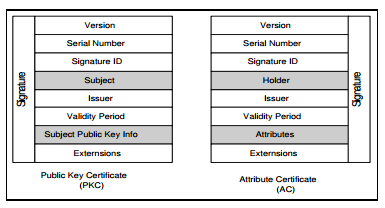
\includegraphics[width=0.5\textwidth]{diff.png}
	\caption{Differences between PKC and AC~\cite{godavari2001secure}}
	\label{fig:diff}
\end{figure}

\subsection{Examples of usage}
An AC can be used in different security related services. "As an example it could also be used to certify authorization information related to a public key. More specifically, it may be used to limit the liability resulting from a digital signature, or to constrain the usage of a public key (e.g., transaction of a limited value, certain time windows, etc.)."~\cite{tilborg2011encyclopedia}.

Different default attributes have been proposed, some of which are listed below.~\cite{benantar2006access,rfc_ac}
\begin{itemize}
	\item \textit{Service Authentication Information}, which identifies the AC holder to the service by name, with optional service-specific authentication information. This attribute could, by using some encryption scheme, also include the holder's identity and password.
	\item \textit{Charging identity}, which is used to charge the holder for the use of services.
	\item \textit{Role}, which is used to specify the role the holder has within a specific service.
	\item \textit{Clearance}, which defines the clearance the holder has for specific information (secret, top-secret, etc.).
	\item \textit{Group}, which describes the group the holder belongs to.
\end{itemize}

More rough examples~\cite{tilborg2011encyclopedia} indicate the use of ACs for DRM-secured devices. ACs could grant applications the right to install itself on devices like iPads and alike.

\subsection{Public Key Infrastructure to fit AC in}
To use ACs within an organisation, there are mainly two implementation defaults, the so called \textit{push} and \textit{pull} models. This paper roughly describes the main arguments for choosing either of the two.

The \textit{push} model requires the AC holder to own his AC. When speaking to the Server, he/she is required to attach the AC with the request. "The 'push' model is suitable in application where the client's permissions should be authenticated/validated in the client's 'home' domain."~\cite{godavari2001secure} This means that no new connections need to be set up between the Server and other parties, as will be in the \textit{pull} model.

The \textit{pull} model requires the Server to retrieve the AC from a repository or an AC issuer. This means the implementation does not involve a change in the client-server protocol, which has benefit over the \textit{push} method when implemented within an existing infrastructure. "The 'pull' model is suitable when the client's priviliges should be authenticated in the inter-domain"~\cite{godavari2001secure} Furthermore, there is no need to update client's ACs when they expire, this can be done within the repository or AC issuer.

\section{Cryptography in Attribute Certificates}
\label{cryptography_in_ac}
This Section describes the role of cryptography within the use of ACs and the way ACs are constructed and issued by an AC issuer. Lets stress again that this section is not ment to give a complete overview of the cryptography involved with ACs.

\subsection{Issueing of an Attribute Certificate}
Within an organisation, there must be a clear seperation between a Certificate Authority (CA) and an Attribute Certificate Authority (AA) as prescribed by the RFC~\cite{rfc_ac}. Within the same organisation the public key of the AA is distributed and trusted, which means that documents signed by the AA are trusted directly and not via a PKC path. An AA can build an AC and sign it using his private key, which can later on be verified by a Server or Service (AC verifier).

After the AC has been build, either the \textit{push} or \textit{pull} model can be used to either distribute the AC to the client, or to distribute it to the AC repository. AC verifiers will verify the validity of an AC for an action or authenticate using the following steps.~\cite{rfc_ac}
\begin{enumerate}
	\item The AC holder's PKC must be present, and the entire certification path of that PKC must be verified.
	\item The AC signature must be cryptographically correct and the issuers PKC certification path must be verified.
	\item The AC issuer must be trusted directly (as mentioned above, the ACs Public Key should be trusted).
	\item The time for which the AC is being evaluated must be within the AC validity.
	\item The AC must follow the standard.
	\item The AC must not contain unsupported critical extensions.
	\item The AC should not have been revoked.
\end{enumerate}

\subsection{Cryptography}
ACs are signed by the AA using a Signature Algorithm which is specified within the AC. The algorithms allowed for the signature are listed in different RFCs~\cite{rfc_alg1,rfc_alg2,rfc_alg3,rfc_alg4}.

\section{Security Requirements}
\label{security_requirements}
What are the security requirements outlined in this RFC? What security problems does it attempt to solve? What (cryptographic) attacks does it defend against?
--> revocation

\bibliographystyle{IEEEtran}
\bibliography{IEEEabrv,literature}
\end{document}






























